\documentclass[a4paper,10pt]{report} % {article}
%\documentclass[a4paper,10pt]{scrartcl}


% ==== Header for document with math =========

% --- input -----------------------------------
  \usepackage[utf8]{inputenc}
  \usepackage[base]{babel}  
  
% --- math -----------------------------------
  \usepackage{amsmath}
  \usepackage{amsfonts}
  \usepackage{amstext}
  \usepackage{amssymb}
  \usepackage{amsthm}
  

% --- graphic and formating ------------------
  % bibliography
  \usepackage[sort,comma]{natbib}
  % settings
  \usepackage{enumitem}
  \usepackage{setspace}
  \usepackage{pdflscape}
  \usepackage{graphicx}
  \usepackage{wrapfig}
  \usepackage[hypcap]{caption}
  \usepackage{subcaption}
  % \usepackage[cm]{fullpage}
  \usepackage[top=2cm, bottom=1.7cm, left=3.6cm, right=1.1cm]{geometry}
  % \usepackage[leftmargin=2.5cm]{geometry}
  %\usepackage{subfigure}
  %\usepackage{caption}
  %\usepackage{subcaption}  
  \usepackage{placeins}
  \usepackage{makeidx} 
  \usepackage{epstopdf}
  % \usepackage{tocloft}     % custom lists
  % \usepackage{minitoc}     % table of content in a chapter
  
   \usepackage{listings}     % code listings
  % \usepackage[printwatermark]{xwatermark} % \usepackage{draftwatermark}
  
  \usepackage[colorlinks=true,linkcolor=interlink,citecolor=DarkCite]{hyperref}
  
  % \usepackage{picture}
  \usepackage[usenames,dvipsnames]{color}
  \usepackage{colortbl} 
  

   \setlength{\headsep}{16pt}
%    
   \usepackage{fancyhdr}
   % ---- fancy page setting -------------- 
   %\input{./latex/style_header_footer.tex}
   \fancyhead[l]{\color{gray}{19. and 21. June 2023}}
\fancyhead[r]{\color{gray}{Informal LaTeX workshop}} % {Exam METABL ~---~ August 1, 2018}
\fancyfoot[l]{\color{gray}{intermediate and advanced topics}}
\fancyfoot[c]{\color{gray}{- \thepage/\pageref*{LastPage} -}}
\fancyfoot[r]{\color{gray}{\( \star \)}} 
\setlength{\headheight}{18pt}
    \renewcommand{\headrulewidth}{1pt}
    \renewcommand{\footrulewidth}{1pt}

   %----------------------------------------
  
  % picture libraries
  \usepackage{tikz} % Required for flow chart
   \usetikzlibrary{arrows,positioning} % Tikz libraries required for the flow chart in the template
   
       \tikzset{
        %Define standard arrow tip
        >=stealth',
        %Define style for boxes
        point/.style={
           rectangle,
           rounded corners,
           draw=black, very thick,
           text width=6.5em,
           minimum height=2em,
           text centered},
        % Define arrow style
        pil/.style={
           ->,
           thick,
           shorten <=2pt,
           shorten >=2pt,}
    }

   \usepackage{csvsimple}  % csv table
   
   \usepackage{lipsum}    % filler text
   
   
  %\hypersetup{
    % bookmarks=false,         % show bookmarks bar?https://www.overleaf.com/project/637266f5927ea984e19f515e
    % unicode=false,          % non-Latin characters in Acrobat’s bookmarks
    % pdftoolbar=false,        % show Acrobat’s toolbar?
    % pdfmenubar=false,        % show Acrobat’s menu?
%     % pdffitwindow=false,     % window fit to page when opened
    % pdfstartview={FitH},    % fits the width of the page to the window 
    %pdfauthor={Author},     % author
    %pdfsubject={Subject},   % subject of the document
    %pdfcreator={Creator},   % creator of the document
    %pdfproducer={Producer}, % producer of the document
    %pdfkeywords={keyword1, key2, key3}, % list of keywords
    % pdfnewwindow=true,      % links in new PDF window
  \hypersetup{
    pdfinfo={
        Title={Informal LaTeX workshop},
        Author={InScAPE group},
        Creator={Your Name Here},
        Producer={Institute for Geophysics and Meteorology},
        Subject={Informal LaTeX workshop on intermediate and advanced topics},
        Keywords={tables, tikz, counters}
    },
    colorlinks=true,            % false: boxed links; true: colored links
    linkcolor= ref_out,         % color of internal links
    linkbordercolor = red,      % color of box around links 
    citecolor=green,            % color of links to bibliography
    filecolor=cyan,             % color of file links
    urlcolor=magenta,           % color of external links
    urlbordercolor = {0 0.6 1}  % (change box color with linkbordercolor)
    % pdfborderstyle={/S/U/W 1} % border style will be underline of width 1pt
} 

% ---- new commands --------------------------
  % ----- link colours ------------
    \newcommand{\reffig}[1]%
    {\hypersetup{linkcolor=figlink}%
    \ref{#1}%
    \hypersetup{linkcolor=interlink}}
 
  % ---- math symbols  ----------------------- 
  \newcommand{\e}{\mathrm{e}}
  \newcommand{\dx}{\mathrm{d}}
  \newcommand{\normal}{\mathbi{n}}
  \newcommand{\bsigma}{\mathbf{t}}
  \newcommand{\vnull}{\mathbf{0} \!\!\! ^{ _{ _{\scriptscriptstyle -}}}}
  \newcommand{\vnullt}{\mathbf{0}^{ \mathrm{T} \!\!\!\!\!\!\! \! _{ _{\scriptscriptstyle -}}}}
  % ---- math fonts -------------------------- 
  \newcommand{\mathbs}[1]{\textsf{#1}}
  \newcommand{\mathbi}[1]{\textbf{\emph #1}}
  \newcommand{\mathff}{\textbf{\textit f}}
  \newcommand{\mathbis}[1]{\textsf{\em #1}}
  \newcommand{\mathcb}[1]{\boldsymbol{\mathcal #1}}
  
  
\newcommand{\thv}{\theta_{\scriptscriptstyle \mathcal{V} }}
\newcommand{\thml}{\theta^{\scriptscriptstyle \mathrm{(ML)}}}

  % --- modifying existing commands -------------------
  

  
  % ---- our own Macros  --------------------------
  
  %  our own lists 
%  \newcommand{\listoflists}{List of Lists}  % we add a list
  
%  \newlistof{lists}{tol}{\listoflists}      % list itself 
  
%  \newcommand{\list}[1]{%
%    \refstepcounter{lists}
%    \par\noindent\textbf{lists \theexample. #1}
%    \addcontentsline{tol}{list}
%    {\protect\numberline{\thechapter.\theexample}#1}\par
  
  

% ---- latex commands -----------------------
  % --- graphic commands --------------------
  \DeclareGraphicsExtensions{.png,.jpg}

  % --- colour definition ------------------
  % colour definition
  \definecolor{GreenDone}{rgb}{0.2,0.7,0.2}
  \definecolor{lightorange}{rgb}{0.9,0.4,0}
  \definecolor{lightestorange}{rgb}{1,0.8,0.5}
  \definecolor{darkorange}{rgb}{0.2,0.1,0}
  \definecolor{interlink}{rgb}{0.6,0,0}
  \definecolor{DarkCite}{rgb}{0,0.3,0}
  % \definecolor{ref_out}{rgb}{0.3,0.3,0}
  \definecolor{ref_out}{rgb}{0.6,0,0}
  \definecolor{lightyellow}{rgb}{0.99,0.99,0.4}
  \definecolor{UeaBlue}{RGB}{0,76,103}
  \definecolor{LightBlue}{RGB}{20,20,250}
  \definecolor{DarkBlue}{RGB}{15,10,100}  
  \definecolor{figlink}{RGB}{45,10,120} 
  \definecolor{bordercol}{RGB}{40,40,40}
  \definecolor{headercol1}{RGB}{186,215,230}
  \definecolor{headercol2}{RGB}{0,76,103}
  \definecolor{headerfontcol}{RGB}{0,0,0}
  \definecolor{boxcolor}{RGB}{186,215,230}

 
\title{Advanced LaTeX Workshop}
\author{Your Name Here}
\date{19 June 2023} 

\pdfinfo{%
  /Title    (Advance LaTeX Workshop) 
  /Author   (Your Name Here)
  /Creator  (Your Name Here)
  /Producer (InScAPE)
  /Subject  (Intermediate and Advanced LaTeX)
  /Keywords (listing, tikz, macrtos) 
}
  
\begin{document}
% later: #4 generating index 
%--------------
%\makeindex
%--------------


% \maketitle
 \pagestyle{fancy}
 
%-------- Workshop overview-------------------------------
 We are organising an informal \textbf{workshop} on the \textbf{intermediate and advanced topics} in \LaTeX.
Although there are various \LaTeX tutorials and templates floating around, but they often omit some tools and packages that are useful in meteorology and geophysics. The workshop is primary focused on PhD students who are starting to write their thesis, but it is open to other \LaTeX users as well.
 \begin{enumerate}
 \item  Monday 19. June --- from 12:45 in CIP room 
 \item  Wednesday 21. June --- from 15:00 in CIP room
\end{enumerate}

\noindent
You can work from CIP workstation or bring your own device.~\\

 \begin{tabular}{l p{0.7\textwidth}}
   target audience: & people with previous experience with \LaTeX \\
   aims:  & discuss \LaTeX ~topics practise skills \\
   duration: & one and half hour from start time or until you start getting tired \\
   topics: & see following sections \ref{sec:monday} and \ref{sec:wednesday} \\
   registration: & comment in this Slack thread \\ 
 \end{tabular}

%-----------------------------------------------------------------------------
 
\section{Monday} \label{sec:monday}

\pagenumbering{arabic} 
\setcounter{page}{1}


\subsection{Combining Document from Pieces}
Combining documents from multiple files speeds up the editing process, makes collaboration easier, and also lowers the risk of accidentally rewriting something. You can see an example how most of the header of this document is in a separate file.
% #1 
To try this, write some dummy text in a separate file and insert is here using the \texttt{input} command:\\
% \input{filename}

% #2 
The \texttt{input} statement can also work on multiple levels
\begin{enumerate}
    \item Make a copy of \texttt{latex/style1headerfooter.tex} and modify it.
    \item Open \texttt{in1header.tex} and replace \texttt{latex/style1headerfooter.tex} with the name of your new file.
    \item Recompile the main document.
\end{enumerate}



\subsection{Automatically Generated Lists}\label{sec:automatic}
There is an easy way how to create list of figures, tables, as well as index of phrases. 

% We are going to start witth this documet
%  #1 change the class of document from article to report
%  


% \maketitle
% \pagenumbering{roman}
%   \let\clearpage\relax 
%   \tableofcontents
%    \label{contents}
%    \addcontentsline{toc}{section}{Table of Contents} %\let\clearpage\relax
%    \addcontentsline{toc}{section}{List of Tables}
%    \listoftables    
%    \addcontentsline{toc}{section}{List of Figures}  %\let\clearpage\relax 
%    \listoffigures
%    \chapter*{List of Symbols}
%    \addcontentsline{toc}{section}{List of Symbols}
%    % ========================
% list  of symbols
%=======================
\begin{onehalfspace}
\begin{tabular}{l l p{0.7\textwidth} }
\hline
		notation  & unit & meaning \\
\hline \\
		\( \sim \) & \( \cdot \) & similar - assignment of probability distribution\\	
		\( \propto \) & \( \cdot \) & proportional equivalent to; i.e.  equivalent up to a constant\\
		\( \overline{(\; \cdot \;)} \) & \( \cdot \) & horizontal averaging \\
		\( \overline{\varphi} \) & 	\( \cdot  \) & mean value of a quantity \( \varphi \)  \\
% 		\( \overline{\varphi}^{(l,k)} \) & 	\( \cdot  \) & mean value of a quantity \( \varphi \) over a subdomain \\		
% 		\( \varphi^{\prime}\) & 	\( \cdot  \) & variant part of a quantity \( \varphi \)  \\			
% 		\( \overline{(\; \cdot \;)}_{u}^{(u)} \) & \( \cdot \) &  averaging over the area of strong updraughts \\
% 		\( {(\; \cdot \;)}_{RE}\) & \(\ \cdot \) &  resolved values of a term in parenthesis\\
% 		\( \overline{(\; \cdot \;)}_{SG}\) & \(\ \cdot \) &  statistics of modelled subgrid values of a term in parenthesis\\	
% 		\( {(\; \varphi \;)}_{(\mathrm{sm}),\lambda}  \) & \( \cdot \) & smoothing of a series of variable \( \varphi \)  over smoothing length \(\lambda \) \\	
% 		
% 		\( \triangle_{\varphi}\) & \( \cdot \)  & perturbation in a quantity \( \varphi \) \\
% 		\\
% 		
% 		\( a_u \) & \( \mathrm{m} \mathrm{s}^{-1}  \) & fraction of the area taken by strong updraughts \\	
% 		
% 		\( C_{p} \)  & \(\mathrm{J} \; \mathrm{kg}^{-1} \, \mathrm{K}^{-1}  \) & specific heat capacity at constant pressure (isobaric mass heat capacity)\\
% 		
% 		\( d_{\mathrm{(h)}} \) & \( \mathrm{m} \) & length of a side of block in a heterogeneity pattern \\			
% 		\( E_{k} \)  & \(\mathrm{J} \; \mathrm{kg}^{-1}  \) & kinetic energy per unit of mass\\
% 		\( E_{w} \)  & \(\mathrm{J} \; \mathrm{kg}^{-1}  \) & kinetic energy of vertical motion\\
% 		\( h^{(\varphi)}_i  \) & \( \cdot \) & scalar flux of the quantity \( \varphi \) \\
% 		\( L_{e} \)  & \(\mathrm{J} \; \mathrm{kg}^{-1} \) & latent heat of evaporation \\
% 		
% 		
% 		\( N \)  & \( \scriptstyle{1} \) & number of gridpoints / number of measurements in a timeseries  \\
% 		\( N_{x} \)  & \( \scriptstyle{1} \) & number of gridpoints in the direction of the axis-\(x\)\\
% 		\( \mathsf{N}(\mu,\sigma^{2}) \)  & \( \cdot \) & normal distribution with mean \( \mu \) and standard deviation \(\sigma \)  \\
% 
% 		\( r \)  & \( \mathrm{kg} \; \mathrm{kg}^{-1} \) & water vapour mixing ratio \\	
% 		%-> do we use this one ?
% 		\( r_{l} \)  & \( \mathrm{kg} \; \mathrm{kg}^{-1} \)  & liquid water mixing ratio\\
% 		\( r_{\varphi} \)  & \( \cdot \)  & residua in a series of the variable \( \varphi \) \\
% 		
% 		\( q_{v} \)  & \( \mathrm{kg} \; \mathrm{kg}^{-1} \) & specific humidity \\
% 		\( q_{cl} \)  & \( \mathrm{kg} \; \mathrm{kg}^{-1}  \)  & cloud total water content \\
% 		\( q_{i} \)  & \( \mathrm{kg} \; \mathrm{kg}^{-1}  \)  & cloud ice water content \\
% 		\( q_{l} \)  & \( \mathrm{kg} \; \mathrm{kg}^{-1}  \)  & cloud liquid water content \\
% 		\( q_{t} \)  & \( \mathrm{kg} \; \mathrm{kg}^{-1}  \)  & total water content (total humidity) \\
% 
% 		\( q_{tr} \)  & \( \; \mathrm{kg}^{-1}  \)  & content of a passive aerosol tracer\\	
% 		
% 		\( Q_{LH} \)  & \( \mathrm{W} \, \mathrm{m}^{-2} \) & latent heat flux \\
% 		\( Q_{SH} \)  & \( \mathrm{W} \, \mathrm{m}^{-2} \)  & sensible heat flux \\
% 		
% 		\( P( A ) \)  & \( \cdot \)  & probability of an event A \\
% 		
% 		\\ \hline
	\end{tabular}
    \end{onehalfspace}

%   \begin{onehalfspace}
%   \begin{tabular}{l l p{0.7\textwidth} }
%   \hline
% 		notation  & unit & meaning \\
% 		\hline \\
% 		\( \mathbb{S}_{i,j} \) & \( \mathrm{s}^{-1} \) & rate of strain tensor \\
% 		\( S \) & \( \mathrm{s}^{-1} \) & modulos of the rate of strain tensor \\
% 		\( S_{\varphi,\alpha} \) & \( \cdot \) &  sample quantile of values of variable \( \varphi \) for probability \(alpha \)\\
% 		
% 		\( t_0 \)  & \( \mathrm{s} \)  & time of transition - when the surface starts warming\\	
% 		\( T \)  & \( \mathrm{K} \)  & absolute temperature\\		
% 		
% 		\( \mathbi{u} \) & \( \mathrm{m} \mathrm{s}^{-1}  \) &  vector of wind velocity  \\
% 		
% 		\( u \) & \( \mathrm{m} \mathrm{s}^{-1}  \) &  component of wind velocity in the direction of axis-\(x\)  \\
% 		
% 		\( \mathsf{U}(a,b) \)  & \( \cdot \) & uniform distribution on the interval \([a,b] \) \\
% 		\( v \) & \( \mathrm{m} \mathrm{s}^{-1}  \) &   component of wind velocity in the direction of axis-\(y\)  \\
% 		\( v_f \) & \( \mathrm{m} \mathrm{s}^{-1}  \) & large scale wind forcing in the direction of  axis-\(y\) \\		
% 		\( w \) & \( \mathrm{m} \mathrm{s}^{-1}  \) &  vertical component of wind velocity \\
% 		
% 		\( w_u \) & \( \mathrm{m} \mathrm{s}^{-1}   \) & vertical velocity in strong updraughts\\
% 		\( \overline{(w^{\prime} \varphi^{\prime})} \) & 	\( \cdot \) & vertical flux of scalar quantity; general notation \\
% 		\( \overline{(w^{\prime} \varphi^{\prime})}_{s} \) & 	\( \cdot \) & vertical flux of scalar quantity at the surface; general notation \\			
% 
% 		\( \overline{(w^{\prime} \theta^{\prime})} \) & 	\( \cdot \) 	& vertical kinematic heat flux \\ % ? adjust name? 
% 		\( \overline{(w^{\prime} \theta^{\prime}_{v})} \) & 	\( \cdot \) 	& vertical kinematic buoyancy flux \\ % ? adjust name? 
% 		\( \overline{(w^{\prime} q^{\prime})} \) & 	\( \cdot \) 		& vertical kinematic moisture flux\\ % ? adjust name ?	
% 		
% 		\( z_{0,\mathrm(vec)} \) 	& \( \mathrm{m}  \) & aerodynamic roughness length\\
% 		\( z_{0,\mathrm(vec)} \) 	& \( \mathrm{m}  \) & aerodynamic roughness length for wind \\
% 		\( z_{0,\theta} \) 		& \( \mathrm{m}  \) & aerodynamic roughness length for scalar quantities\\
% 		\( z_i \) & \( \mathrm{m}  \) & height of the mixed boundary layer (MBL) \\	
% 		\( \mathsf{z}_{\alpha} \) & \scriptsize{1}  &   quantile of the standard normal distribution for probability \(\alpha\)\\
% 		
% 		\( \delta_{i,j} \) &  \scriptsize{1} & Kronecker delta\\
% 		
% 		%-> change this one?
% 		\( \delta_{\mathrm{(h)}} T \) & \( \mathrm{K} \) & temperature scale of a heterogeneity in surface potential temperature\\
% 		\( \delta t \) & \( \mathrm{s} \) & length of timestep in a timeseries \\
% 		\( \Delta t \) & \( \mathrm{s} \) & length of a  timestep of numerical computations \\
% 		\( \Delta x \) & \( \mathrm{m} \) & grid resolution in the direction of x-axis \\
% 		\( \Delta z \) & \( \mathrm{m} \) & grid resolution in the vertical direction \\		
% 		\( \Delta_{\mathrm{(h)}} T \) & \( \mathrm{K} \) & temperature scale of a surface anomaly \\
% 		%-> check this one		
% 		\( \varepsilon_{i,j,k} \) &  \scriptsize{1} & Levi-Civita symbol in three dimensions\\
% 		\( \theta \)  & \( \mathrm{K} \)  & potential temperature \\
% 		\( \theta_{e} \)  & \( \mathrm{K} \)  & equivalent potential temperature \\		
% 		% \( \theta_{v} \)  & \( \mathrm{K} \)  & virtual potential temperature \\
% 		% \( \theta \)  & \( \mathrm{K} \)  & potential temperature \\
% 		\( \theta_{\mathrm{surf}} \) & \( \mathrm{K} \) & surface potential temperature\\	
% 		\( \theta_{v} \)  & \( \mathrm{K} \)  & virtual potential temperature \\
% 	      \\ \hline
% 	\end{tabular}
%       \end{onehalfspace}

%       \begin{onehalfspace}
%       \begin{tabular}{l l p{0.7\textwidth} }
% 	    \hline
% 	    	notation  & unit & meaning \\
% 	    \hline \\
% 		\( \kappa \) & \scriptsize{1} & Von Kármán constant \\
% 
% 
% 		\( \lambda \) & \( \mathrm{m} \) & mixing length \\
% 		\( \lambda_0 \) & \( \mathrm{m} \) & reference mixing length \\		
% 		\( \nu_m \) & \( \mathrm{m}^{2} \mathrm{s}^{-1}\)  & sub-filter eddy-viscosity in a subgrid model \\
% 		\( \nu_{m,s}\) & \( \mathrm{m}^{2} \mathrm{s}^{-1}\)  & sub-filter eddy-viscosity in the surface exchange model \\
% 		\( \nu_h \) & \( \mathrm{m}^{2} \mathrm{s}^{-1}\)  & sub-filter eddy-diffusivity in a subgrid model \\
% 		\( \nu_{h,s} \) & \( \mathrm{m}^{2} \mathrm{s}^{-1}\)  & sub-filter eddy-diffusivity in a surface exchange model\\
% 		
% 		\( \sigma_{\varphi} \)  & \( \cdot \) & standard deviation of a quantity \( \varphi \) \\	
% 		
% 		\( \varphi \) & 	\( \cdot  \) & scalar quantity; general notation \\
% 		\( \rho \)  & \( \mathrm{kg} \; \mathrm{m}^{-3} \) & density of air \\	
% 		\( \tau \)  & \( \mathrm{N} \, \mathrm{m}^{-2} \)  & vertical momentum flux; wind stress\\
% 		\( \tilde{\tau}_{i,j} \)  & \( \mathrm{N} \, \mathrm{m}^{-2} \)  & tensor of the subgrid stress\\
% 		\( \phi_m \) &  \scriptsize{1} & Businger--Dyer function for the momentum \\
% 		\( \phi_h \) &  \scriptsize{1} & Businger--Dyer function for the heat flux \\
% 	
% 	
% 		% add a note about vertical fluxes - always upward
% 		
% \\ \hline
% 	\end{tabular}
% \end{onehalfspace}

%\newpage
\section*{List of Abbreviations}
\addcontentsline{toc}{section}{List of Abbreviations}

\begin{onehalfspace}
	\begin{tabular}{l p{0.7\linewidth}}
\hline
		notation & meaning \\
\hline \\
		% AtTW 	&   after the tranisition to warm surface conditions \\  %-> add this one
		AWS	& automatic weather station \\
		%d->? or automated   - NO		
		ABL 	& atmospheric boundary layer \\
		CAO 	& cold--air outbreak \\
		CBL 	& convective boundary layer \\
% 		CFL	& Courant-Friedrichs-Lewy condition \\
% 		Cu      & cumulus \\
% 		CuL 	& cumulus layer \\
% 		EDMF	& eddy-diffusivity mass-flux \\
% 		IBL	& internal boundary layer \\
% 		IFS	& ECMWF Integrated Forecasting System \\
% 		%d -> check whether it is correct IQR : corrected
% 		IQR	& interquartile range \\
% 		EZ 	& entrainment zone \\
% 		FA 	& free atmosphere \\
% 		LES	& large eddy simulation \\
% 		LEM	& Met Office Large Eddy Model \\
% 		LH	& latent heat \\
% 		LW	& long-wave infrared radiation \\
% 		MetUM	& Met Office Unified Model \\	
% 		MIZ	& marginal sea-ice zone \\
% 		ML 	& (well-) mixed layer \\
% 		P--W	&  Piascek--Williams \\
% 	        %-> keep this one
% 		CtS 	& control set \\
		SBL 	& stable boundary layer \\
		Sc 	& stratocumulus\\
		SH	& sensible heat \\
		TKE	& turbulent kinetic energy \\
\hline
	\end{tabular}
\end{onehalfspace}


% \newpage

%\chapter{Monday} 


 \subsection{Modifying Plots and Schematics}\label{sec:figures}
 %\newpage
 %\thispagestyle{empty}
 \begin{figure}[h!] 
     %     % tikz diagram
     \begin{tikzpicture}[node distance=7mm, auto,]
        %nodes
        \node[point] (market) { \nameref{sec:automatic} };
        \node[point, inner sep=5pt,below=0.5cm of market]
        (conference) {Conferences (see \ref{sec:automatic})};
        % We make a dummy figure to make everything look nice.
        \node[above=of market] (dummy) {};
        \node[right=of dummy] (t) {Poster template}
        edge[pil,bend left=45] (market.east) % edges are used to connect two nodes
        edge[pil, bend left=45] (conference.east); % .east since we want
                                                    % consistent style
        \node[left=of dummy] (g) {Feedback}
        edge[pil, <-,bend right=45] (market.west)
        edge[pil,->, bend left=45] node[auto] {Poster Idea \pageref{fig:standalone} } (t);
    \end{tikzpicture}~\hspace{-2ex}

      \begin{tikzpicture}[node distance=8mm, auto,]
        %nodes
        \node[point] (market) {users (b)};
        \node[point, inner sep=5pt,below=0.5cm of market]
        (conference) {Conferences (c)};
        % We make a dummy figure to make everything look nice.
        \node[above=of market] (dummy) {};
        \node[right=of dummy] (t) {Poster template}
        edge[pil,bend left=45] (market.east) % edges are used to connect two nodes
        edge[pil, bend left=45] (conference.east); % .east since we want
                                                    % consistent style
        \node[left=of dummy] (g) {Feedback}
        edge[pil, <-,bend right=45] (market.west)
        edge[pil,->, bend left=45] node[auto] {Poster Idea (a)} (t);
    \end{tikzpicture}~\hspace{-2ex}
    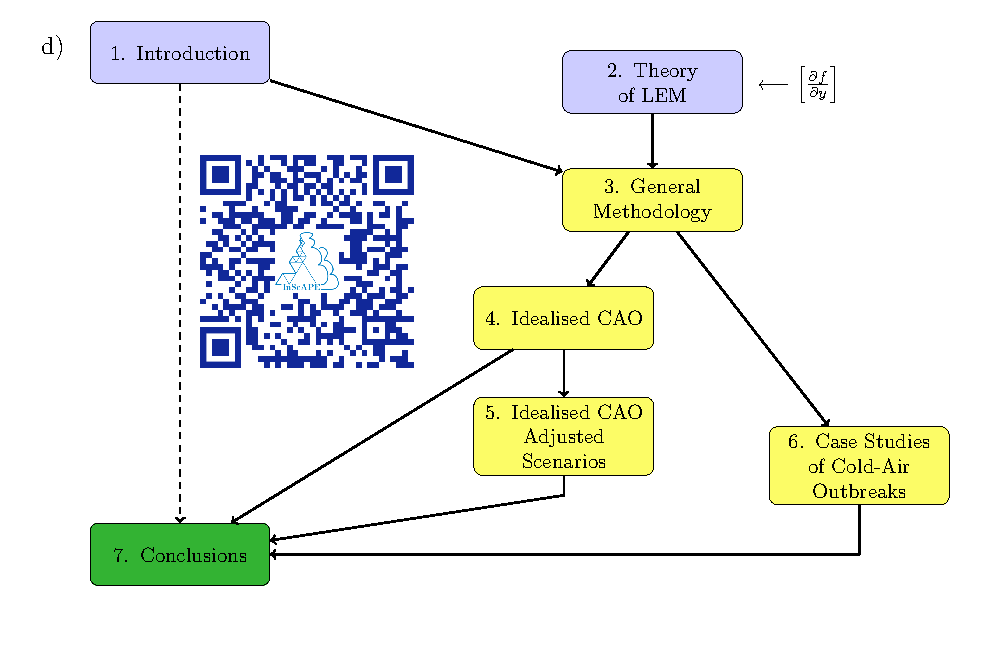
\includegraphics[width=0.7\textwidth]{./figures/standalone.pdf}
        \caption[Diagrams and plots]{Here we combine a \textbf{Tikz} diagrams and images. We can also compile the figure as separate \textbf{standalone} \index{standalone} pdf and then include it as a graphical element. }  
      \label{fig:standalone}
 \end{figure}
 
 %\setcounter{subsection}{7}
 \subsection{Counters}\label{sec:counters}
How did we suddenly jump from section \ref{sec:figures} to \ref{sec:counters}  ?

 \newpage 
 
 \subsection{Customizing Links, References, and Citations}
 Such as modifying the style of links to other parts of the same document (\nameref{sec:automatic}) and links to \href{https://geomet.uni-koeln.de/en/}{external websites}.
 
 
 \subsection{Version Control and Comparison}
 We also look at the external tools such as \texttt{latexdiff} that compares two \LaTeX files, and  \texttt{pdfdiff} that compares \( \ldots \) you know what.   
  


\section{Wednesday} \label{sec:wednesday} 
\subsection{Code Listing with Highligths}
Such as showing a lines from external script or showing the code of this page.
\lstinputlisting[ language={[latex]tex},                     % tex syntax, latex option
  firstline=93, firstnumber=93, lastline=99, numbers=left,
  breaklines=true, basicstyle=\scriptsize, frame=single,
  keywordstyle=\color{magenta}, commentstyle=\color{gray}  % comments are gray colour
]{./latex/day2latex_backup.tex} 

\subsection{Tables} \label{sec:tables}
Instead of copy \& paste values into tables, we just read them from an external csv file and format them.  

\begin{center} 
\csvreader[
        tabular = |r|r|r|, 
        table head  = \hline \( \quad  z \; \lbrack \mathrm{m} \rbrack  \) &  \(  \; \bar{u} \;  \lbrack \mathrm{m\, s}^{-1} \rbrack \)& \(  \quad \quad \Big. \bar{ \theta }  \; \lbrack \mathrm{K} \rbrack \Big. \) \\\hline ,
        table foot = \hline & \multicolumn{2}{ c|}{\( \ldots \) } \\ \hline
        ]{values.csv}
        {z=\zvec, u=\uvec, theta=\thvec}{%
            \zvec  & \uvec & \thvec 
        }% 
\end{center} ~\vspace{1ex}
And the we will further style-up the table. 

\subsection{More on Macros} 
 We can define shortcuts for symbols such as \(\thml\), but we can even write conditional statements.
 
 \subsection{Posters and Slideshows} 
 If you have been struggling with Powerpoint, there is a way out \( \ldots \) 
 
 \section{Dummy section}
 \lipsum[2-7]    %generates dummy text
 
 
% #4 generating index 
%   \clearpage
%   \phantomsection 
%   \addcontentsline{toc}{section}{Index}  
%   \label{index}  
%   Longer documents sometimes include index pages.
%   \printindex  
 
\label{LastPage}
\newpage


\end{document}
